% Created 2014-04-11 Fri 16:59
\documentclass[11pt]{article}
\usepackage[utf8]{inputenc}
\usepackage[T1]{fontenc}
\usepackage{fixltx2e}
\usepackage{graphicx}
\usepackage{longtable}
\usepackage{float}
\usepackage{wrapfig}
\usepackage{rotating}
\usepackage[normalem]{ulem}
\usepackage{amsmath}
\usepackage{textcomp}
\usepackage{marvosym}
\usepackage{wasysym}
\usepackage{amssymb}
\usepackage{hyperref}
\tolerance=1000
\usepackage{epstopdf}
\author{Kuiper, J. \and Marshall I.J. \and Wallace, B.C. \and Swertz M.A.}
\date{\today}
\title{Spá: a web-based viewer for PDF text mining}
\hypersetup{
  pdfkeywords={},
  pdfsubject={},
  pdfcreator={Emacs 24.4.50.1 (Org mode 8.2.5h)}}
\begin{document}

\maketitle
\begin{abstract}
When doing sentence extraction or document level predictions on unstructured text the results of trained models are often hard to interpret within the context of the documents at hand.
Furthermore presenting results to end users can be a considerable user interface challenge.
To this end we present Spá, a generic web-based visualizer for sentence and document level classifiers on unstructured PDF documents.
Spá allows the results of sentence extractions to be visualized within the PDF document itself, and allows other results to be presented alongside it.
\end{abstract}

\section{Introduction}
\label{sec-1}
Finding sentences or words with particular characteristics within a larger document is an important task in natural language processing and machine learning.
For example, one may wish to identify the most important sentences in a document to automatically generate a summary, or extract words that match a certain ontology.
\section{Architecture}
\label{sec-2}
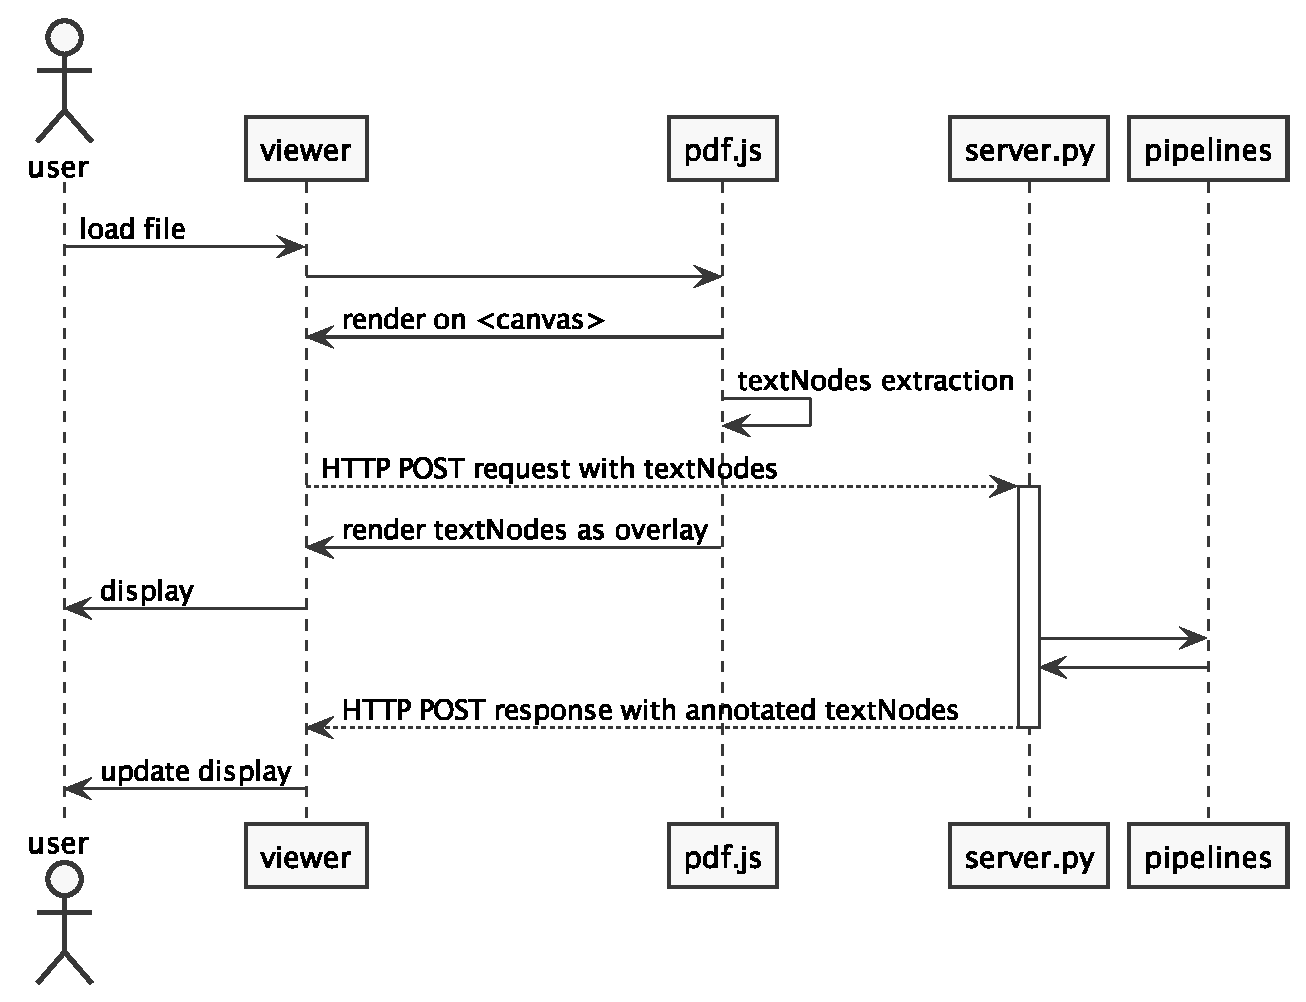
\includegraphics[width=.9\linewidth]{sequence_diagram.eps}
\section{Case Study}
\label{sec-3}
\section{Discussion \& Future work}
\label{sec-4}
% Emacs 24.4.50.1 (Org mode 8.2.5h)
\end{document}
